% --------------------------------------------------------------------------
% Template for DCASE 2026 technical reports; to be used with:
%          dcase2026_techrep.sty  - DCASE 2026 LaTeX style file, and
%          IEEEbib.bst - IEEE bibliography style file.
% Adapted from spconf.sty and waspaa15.sty
% --------------------------------------------------------------------------

\documentclass{article}
\usepackage{dcase2026_techrep,amsmath,graphicx,url,times,booktabs, tabularx}
\usepackage[T1]{fontenc}
\usepackage{xcolor}
\usepackage{booktabs} % For better table formatting
\usepackage{array} % For vertical centering
\usepackage{multirow} % For spanning rows
% Example definitions.
% --------------------
\def\defeqn{\stackrel{\triangle}{=}}
\newcommand{\symvec}[1]{{\mbox{\boldmath $#1$}}}
\newcommand{\symmat}[1]{{\mbox{\boldmath $#1$}}}

% Title.
% --------------------
\title{SRP 16-band UpLAM with Mask R-CNN for audiovisual SELD}

% Single addresses (uncomment and modify for single-address case).
% --------------------
% \name{Author(s) Name(s)\thanks{Thanks to XYZ agency for funding.}}
% \address{Author Affiliation(s)}
%
% For example:
% ------------
% \address{School\\
%       Department\\
%       Address}

% Two addresses
% --------------------
% \twoauthors
%   {John Doe\sthanks{Thanks to ABC agency for funding.}}
%     {Fictional University\\
% Computer Science Dept., 2133 Long Road\\
%      Gotham, NY 10027, USA \\
%      john@fictional.edu}
%   {Maria Ortega\sthanks{Thanks to XYZ agency for funding.}}
%     {  University of the Imagination \\
%      Big Engineering Building, 8765 Dream Blvd. \\
%      New Chicago, IL 60626, USA \\
%      maria@imagination.edu}

% Authors in two lines, use in case of many authors with many affiliations (uncomment and modify).
% --------------------
\name{Rafał Foltyniewicz$^{1}$,
      Rafał Kaczmarek$^{1}$,
      Michał Olejnik$^{1}$,
      Iwan Ryzenkow$^{1}$,
      Bogdan Jastrzębski$^{1}$, 
      }
      %fixed *.sty to allow names on multiple lines
\address{$^1$ Samsung Research Poland, \\\{r.foltyniewi, r.kaczmarek, m.olejnik2, i.ryzenkow, b.jastrzebsk\}@samsung.com\\          
 }

% \name{John Doe$^{1}\sthanks{Thanks to ABC agency for funding.}$,
%       Maria Ortega$^{1}\sthanks{Thanks to XYZ agency for funding.}$,
%       Maria Doe$^{2}$, 
%       John Ortega$^{2}$,
%       John Maria$^{3}$, 
%       }
% \secondlinename{	  
%       David Smith$^{2}$, 
%       Maria Smith$^{3}$,
%       }
%       % fixed *.sty to allow names on multiple lines
% \address{$^1$ Fictional University, Computer Science Dept., Gotham, USA, \{john, maria\}@fictional.edu\\          
%         $^2$ University of the Imagination, Computer Science Dept., New Chicago, USA, \\
%         \{maria, john, david\}@fictional.edu\\ 
%         $^3$ University of the Fantasy, Department of Electronics, Pittsburgh, USA, 
%         \{john, maria\}@fantasy.edu\\
%  }

\begin{document}

\ninept
\maketitle

\begin{sloppy}

\begin{abstract}
We present an audiovisual sound event localization and detection system based on a modified Mask R-CNN with a ResNet-50 Feature Pyramid Network backbone, taking 19-channel inputs composed of 3 RGB video channels and 16 UpLAM acoustic feature maps extracted from the tetrahedral microphone array. The model is trained with progressive backbone unfreezing, class-balanced sampling with inverse-frequency weights (cap=30), focal loss, and data augmentation including azimuth rotation, horizontal flip, RGB dropout, and audio band masking.
\end{abstract}

\begin{keywords}
One, two, three, four, five
\end{keywords}


\section{Introduction}
\label{sec:intro}

DCASE 2026 Task 3 advances sound event localization and detection (SELD) through semantic acoustic imaging, focusing on the integration of spatial audio and audiovisual scenes. This challenge emphasizes the development of robust systems capable of identifying and localizing sound events in complex acoustic environments.

This report outlines the technical approach for participating in challange with the primary aim of redesigning the UpLam model to operate with 16 perceptually relevant Mel frequency bands and leveraging AudibleLight for scalable synthetic data generation.

% \textbf{Please note that headers for challenge and workshop submissions have different header.} Use the appropriate template!




\section{System Architecture and Modifications}
\label{sec:format}
\textcolor{red}{Iwan: baseline default UpLam and modyfied Mask R-CNN}\\
\\
\textcolor{red}{Rafal: modyfied UpLam}



\section{Synthetic Data Generation}
\label{sec:pagelimit}
Given the growing use of synthetic data across different machine learning tasks and the limited amount of data in the original STARSS23 dataset, we chose to use AudibleLight to generate additional data.

AudibleLight is a Python package that provides a unified API for generating synthetic soundscapes through ray-traced simulations and parametric room impulse responses (RIRs). It integrates frameworks like SpatialScaper, SoundSpaces, and Pyroomacoustics to ensure scalable acoustic diversity.

For the generation process, we set parameters to include 5 to 20 static events per 60-second scene, with no moving events. The maximum overlap was set to 4, and the reference decibel level was -50 dB. Events were positioned between 0.5 to 3 meters from the microphone, with a height limit of 0.3 meters relative to the microphone position, which was randomly chosen within a randomly selected mesh. We used the Eigenmike32 mic array, with video resolution set to 1920 x 960 pixels at 10 fps. There was a 50\% chance of adding noise, randomly selected from available options, and the video low power mode was disabled to maintain higher quality meshes.

After generation, the audio was resampled to 24 kHz and 4 appropriate tetrahedral channels were selected. The video was resized to 360:180 resolution, with frames saved as PNG files to meet task specifications.This process produced 122 recordings, totaling in 2 hours and 2 minutes of synthetic data, which were then combined with the original train split of the STARSS23 dataset.

% For some generated scenes there was a texture missing, resulting in black and white video.


% Below is an example of how to insert images. 
% -------------------------------------------------------------------------
% \begin{figure}[t]
%   \centering
%   \centerline{\includegraphics[width=\columnwidth]{fig1a}}
%   \caption{Example of a figure with experimental results.}
%   \label{fig:results}
% \end{figure}

\section{A Note on Numerical Approaches to LAM}
\label{sec:solver}

The LAM pipeline relies on APGD-computed acoustic intensity maps as ground truth for training. We investigated whether exact numerical solvers (Chambolle-Pock, subgradient descent, ADMM) could produce improved estimates. Figure~\ref{fig:solvers} shows representative reconstructions on real LOCATA Eigenmike recordings.

\begin{figure}[t]
  \centering
  \centerline{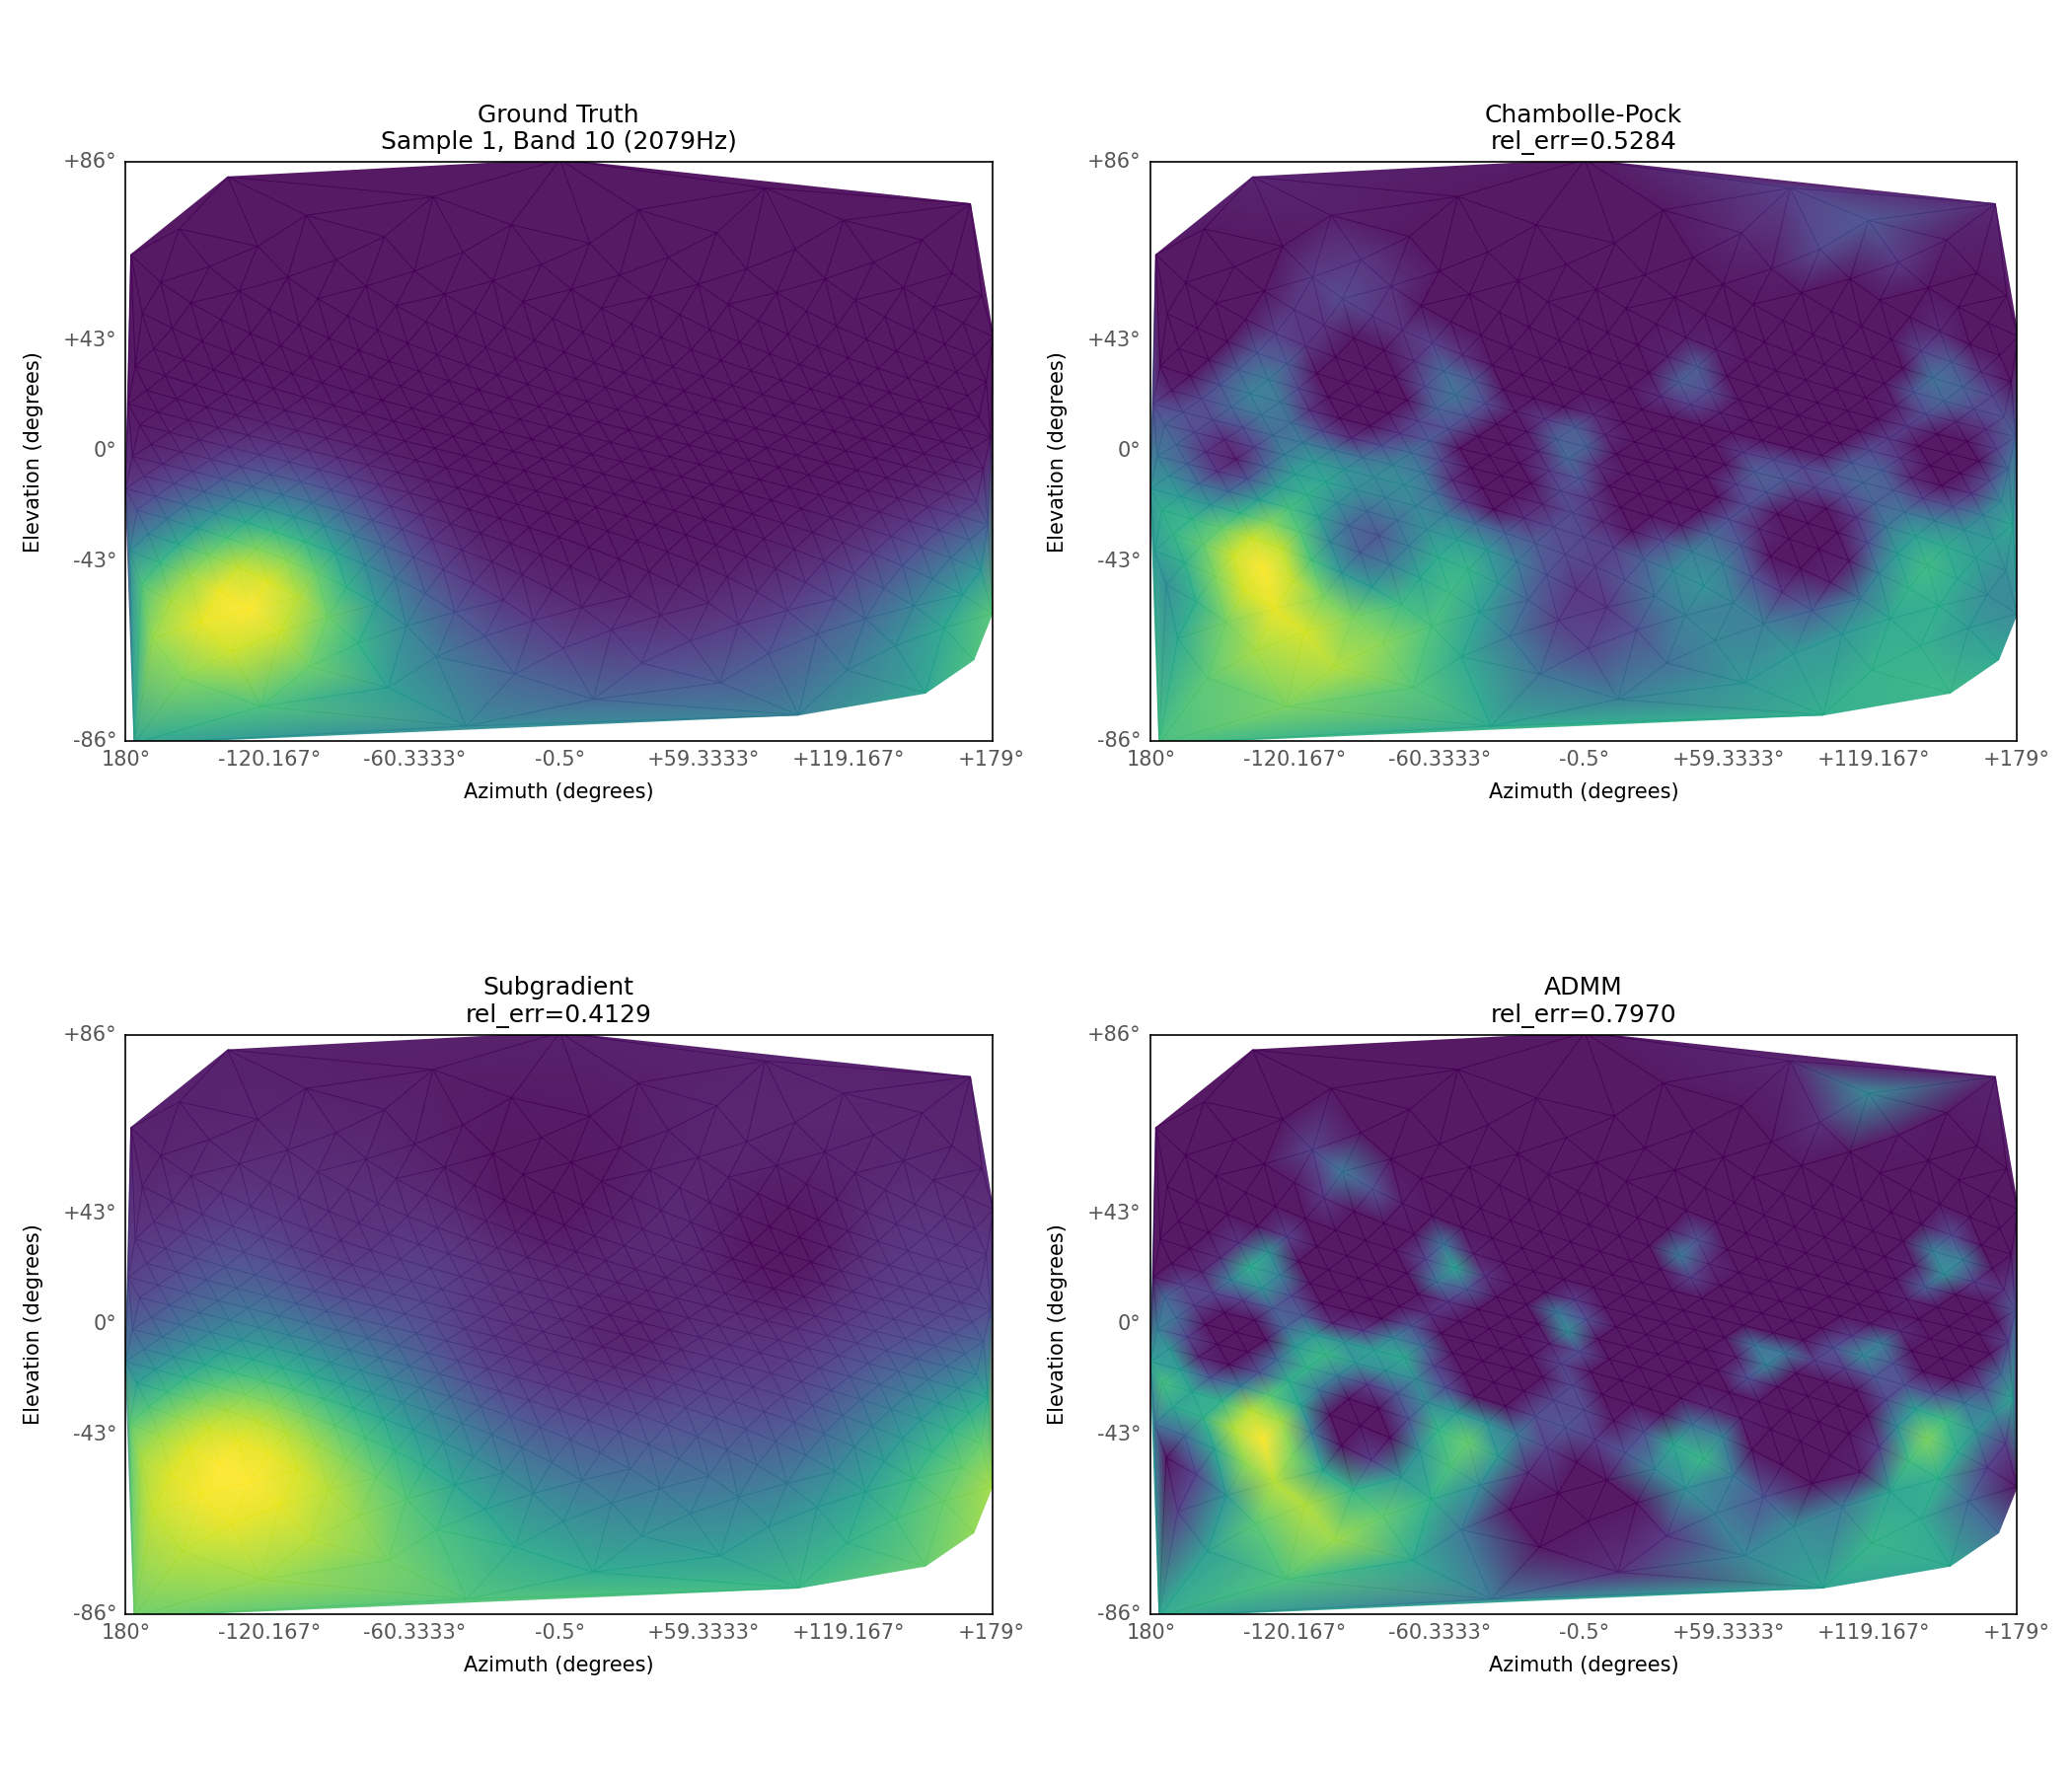
\includegraphics[width=\columnwidth]{viz_sample01_band10.png}}
  \caption{Acoustic map reconstructions on LOCATA data. Chambolle-Pock and ADMM converge to the exact minimizer but exhibit checkerboard artifacts. Subgradient descent and the APGD ground truth remain smooth due to early stopping.}
  \label{fig:solvers}
\end{figure}

ADMM successfully recovers the dominant acoustic source, confirming the mathematical validity of the imaging operator. However, the Hessian $H_{ij}=|a_i^H a_j|^2$ is singular: with 32 microphones mapping onto 484 spatial directions at sub-wavelength resolution, the system is fundamentally underdetermined. Adding quadratic regularization renders the problem well-posed, enabling convergence within tens of iterations.

The true minimizer of the loss, however, exhibits characteristic checkerboard and ringing artifacts (Fig.~\ref{fig:solvers}). ADMM, as the solver that achieves the lowest objective value, reveals these artifacts most clearly. The APGD-based ground truth used in the LAM pipeline produces smooth, visually plausible maps precisely because it is stopped early, before reaching this minimizer. The regularizer promotes piecewise constancy and sparsity but does not encode the physical structure of compact, contiguous acoustic sources on the sphere.

This has implications for training: the LAM model learns to replicate APGD's early-stopped estimates, which are smooth approximations to a loss function whose exact solution does not correspond to the desired acoustic map.

A further consequence is that early stopping precludes warm-starting across consecutive frames. In principle, since acoustic scenes change slowly, the solution from one time frame provides an excellent initialization for the next. This would amortize solver cost: rather than running hundreds of iterations per frame, a handful of fine-tuning steps would suffice, making exact solvers practical for streaming applications. However, if we rely on early stopping to suppress artifacts, warm-starting becomes self-defeating: it accelerates convergence toward the exact minimizer, which is precisely what early stopping was designed to avoid. Maintaining both a running estimate and artifact-free maps would require a frame-dependent stopping rule calibrated to the distance already traveled—an open problem under the current objective.

\section{Experimental Methodology and Results}
\label{sec:pagestyle}
\textcolor{red}{Rafal: training process, parameters, unfreezing etc. GPU? epoch time?}\\
\textcolor{blue}{Rafal F: modyfications in inference}\\
Evaluation dataset\\
Metrics\\
metrics\\

\begin{table*}
\centering
\caption{Example Table with Macro and Micro Evaluation Metrics}
\label{tab:example}
\begin{tabular}{lcccccc}
\toprule
\textbf{Run Name} & \textbf{Metric} & \textbf{AP@0.25} & \textbf{AP@0.5} & \textbf{AP@0.75} & \textbf{mAP} & \textbf{Pearson r} \\
\midrule
\midrule
\multirow{2}{*}{Baseline} & Macro & 0.0010 & 0.0000 & 0.0000 & 0.0003 & 0.1358 \\
& Micro & 0.0032 & 0.0000 & 0.0000 & 0.0011 & 0.4429 \\
\midrule
\multirow{2}{*}{SRP-UPL-MRCNN} & Macro & \textbf{0.0277} & \textbf{0.0069} & \textbf{0.0001} & \textbf{0.0116} & 0.2796 \\
& Micro & 0.0279 & 0.0072 & \textbf{0.0001} & 0.0117 & 0.4270 \\
\midrule
\multirow{2}{*}{SRP-UPL-MRCNN-2} & Macro & 0.0025 & 0.0000 & 0.0000 & 0.0009 & \textbf{0.3455} \\
& Micro & 0.0112 & 0.0000 & 0.0000 & 0.0037 & 0.4189 \\
\midrule
\multirow{2}{*}{SRP-UPL-MRCNN-3} & Macro & 0.0212 & 0.0046 & 0.0000 & 0.0086 & 0.3287 \\
& Micro & \textbf{0.0308} & \textbf{0.0080} & 0.0000 & \textbf{0.0129} & \textbf{0.4791} \\
\midrule
\multirow{2}{*}{SRP-UPL-MRCNN-3} & Macro & 0.0012 & 0.0000 & 0.0000 & 0.0004 & 0.3352 \\
& Micro & 0.0025 & 0.0001 & 0.0000 & 0.0009 & 0.4624 \\
\bottomrule
\end{tabular}
\end{table*}

\section{Conclusion and Future Directions}
\label{sec:majhead}
\textcolor{red}{Bogdan: UpLam training approach}\\
more bands in uplamm good!\\
synthetic data maybe good\\
low mAP, ok pearson?\\
% -------------------------------------------------------------------------
% Either list references using the bibliography style file IEEEtran.bst
\bibliographystyle{IEEEtran}
\bibliography{refs}

or list them by yourself
\begin{thebibliography}{9}

\bibitem{dcase2016web}
  \url{http://www.cs.tut.fi/sgn/arg/dcase2016/}.

\bibitem{IEEEPDFSpec}
  {PDF} specification for {IEEE} {X}plore$^{\textregistered}$,
  \url{http://www.ieee.org/portal/cms_docs/pubs/confstandards/pdfs/IEEE-PDF-SpecV401.pdf}.

\bibitem{PDFOpenSourceTools}
  Creating high resolution {PDF} files for book production with 
  open source tools, 
  \url{http://www.grassbook.org/neteler/highres_pdf.html}.

\bibitem{eWilliams1999}
E. Williams, \emph{Fourier Acoustics: Sound Radiation and Nearfield Acoustic
  Holography}. London, UK: Academic Press, 1999.

\bibitem{ieeecopyright}
  \url{http://www.ieee.org/web/publications/rights/copyrightmain.html}.

\bibitem{cJones2003}
C. Jones, A. Smith, and E. Roberts, ``A sample paper in conference
  proceedings,'' in \emph{Proc. IEEE ICASSP}, vol. II, 2003, pp. 803--806.

\bibitem{aSmith2000}
A. Smith, C. Jones, and E. Roberts, ``A sample paper in journals,'' 
  \emph{IEEE Trans. Signal Process.}, vol. 62, pp. 291--294, Jan. 2000.

\end{thebibliography}


\end{sloppy}
\end{document}

